%!TEX root = main.tex
%%%%%%%%%%%%%%%%%%%%%%%%%%%%%%%%%%%%%%%%%%%%%%%%%%%%%%%%%%%%%%%%%%%%%%%%%%%%%%%%

\section{Introduction}
\label{sec:introduction}

Today, HTTP Adaptive Streaming (HAS) is the dominant way of video delivery in the Internet. 
HAS is based on the wide-spread HTTP protocol and takes over its properties such as easy traversal of NAT-devices, firewall-friendliness, encryption in the shape of HTTPS and close-to-customer caching through content-delivery networks (CDNs).
In HAS, the video content is split into short chunks, e.g. 2 seconds, and each chunk is encoded into different quality levels.
The individual chunks are then made available on standard HTTP servers.
The location of the chunks and their encoding are given to the client through a manifest file.
At beginning of the playback, the streaming client first requests the manifest file. 
Afterward, it chooses the chunks according to its internal adaptation logic, for example based on current throughput or buffer level.
Dynamic Adaptive Streaming of HTTP (DASH) is an ISO standard which defines the structure and content of such a manifest file and is deployed by major content providers such as YouTube or Netflix.






mot1: growth of (adaptive) video streaming

mot2: with the growing competition in video streaming services, user expectations are also growing. Further, it is well known that stalling events and the video encoding bitrate (i.e. the video resolution) have a significant impact on the Acceptance Rate and the QoE \cite{casas2012youtube}.

what:

how

main contribution: we show there there is a lot of room for optimization for the used adaptation algorithms. Even if we completely avoid stalling events, a higher mean video quality is achievable in most cases. The number of resolution switches can be reduced.

structure


\begin{figure}[t]
\centering
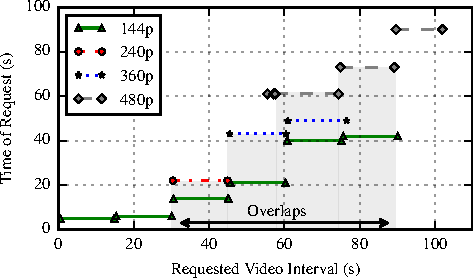
\includegraphics[width=0.9\linewidth]{figs/eg_request_schedule}%
\caption{Request schedule TODO: remake figure}
\label{fig:request_schedule}%
\end{figure}

\cite{sieber16sacrificing,sieber15costaggressive}